\documentclass[11pt]{article}


\usepackage{fullpage}
\usepackage{graphicx}
\usepackage{amsmath}
\usepackage{amssymb}
\usepackage{amsthm}
\usepackage{fancyvrb}

\newcommand{\myname}{Mehshan Mustafa}

\newenvironment{theorem}[2][Theorem]{\begin{trivlist}
\item[\hskip \labelsep {\bfseries #1}\hskip \labelsep {\bfseries #2.}]}{\end{trivlist}}
\newenvironment{lemma}[2][Lemma]{\begin{trivlist}
\item[\hskip \labelsep {\bfseries #1}\hskip \labelsep {\bfseries #2.}]}{\end{trivlist}}
\newenvironment{exercise}[2][Exercise]{\begin{trivlist}
\item[\hskip \labelsep {\bfseries #1}\hskip \labelsep {\bfseries #2.}]}{\end{trivlist}}
\newenvironment{problem}[2][Problem]{\begin{trivlist}
\item[\hskip \labelsep {\bfseries #1}\hskip \labelsep {\bfseries #2.}]}{\end{trivlist}}
\newenvironment{question}[2][Question]{\begin{trivlist}
\item[\hskip \labelsep {\bfseries #1}\hskip \labelsep {\bfseries #2.}]}{\end{trivlist}}
\newenvironment{corollary}[2][Corollary]{\begin{trivlist}
\item[\hskip \labelsep {\bfseries #1}\hskip \labelsep {\bfseries #2.}]}{\end{trivlist}}
\newenvironment{solution}{\begin{proof}[Solution]}{\end{proof}}
\newenvironment{idea}[2][Proof Idea.]{\textit{#1} #2}



\parindent0in
\pagestyle{plain}
\thispagestyle{plain}

\newcommand{\dated}{\today}
\newcommand{\token}[1]{\langle \text{#1} \rangle}

\begin{document}

\textbf{Introduction to the Theory of
Computation}\hfill\textbf{\myname}\\[0.01in]
\textbf{Chapter 2: Context-Free Languages}\hfill\textbf{\dated}\\
\smallskip\hrule\bigskip

\begin{problem}{2.46}
Consider the following CFG $G$:
\begin{align*}
S &\rightarrow SS \ | \ T \\
T &\rightarrow aTb \ | \ ab
\end{align*}
Describe $L(G)$ and show that $G$ is ambiguous. Give an unambiguous grammar $H$ where $L(H) = L(G)$ and sketch a proof that $H$ is unambiguous.
\end{problem}

\begin{problem}[Part]{a}
Describe $L(G)$.
\end{problem}

Let $A = \{a^nb^n \ | \ n \geq 1\}$, then $L(G) = \{w \ | \ w \in A^+\}$.

\begin{problem}[Part]{b}
Show that $G$ is ambiguous.
\end{problem}

Then CFG $G$ is ambiguous, because the string $ababab$ is a member of $L(G)$ and it has more than 1 parse trees in $G$.

\begin{center}
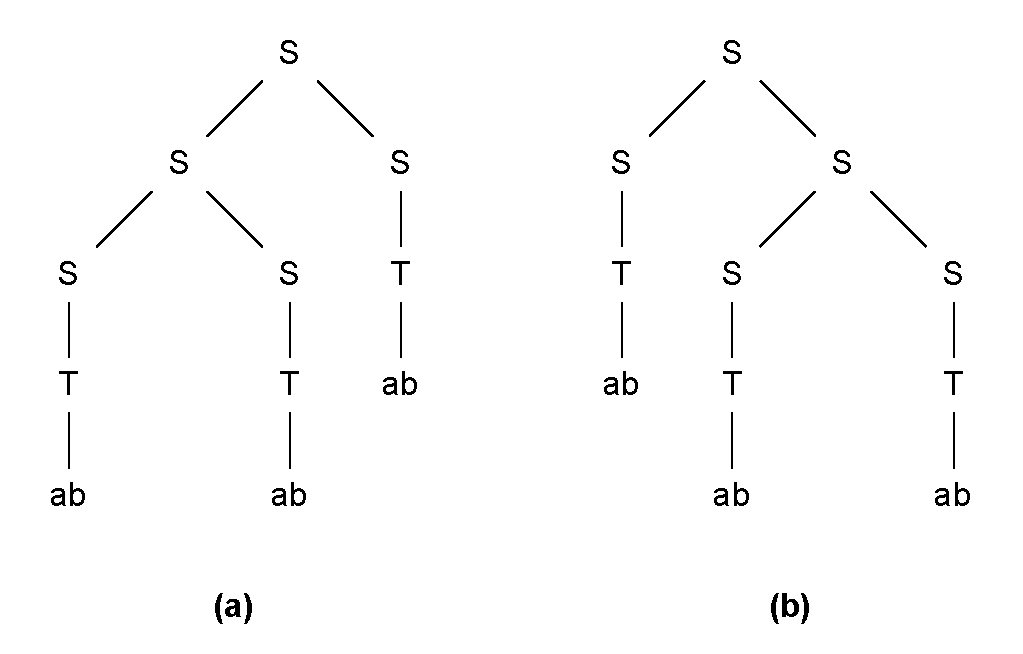
\includegraphics[scale=0.8]{Figures/Problem2.46a.pdf} \\
Two parse trees of the string $ababab$.
\end{center}

\begin{problem}[Part]{c}
Give an unambiguous grammar $H$ where $L(H) = L(G)$.
\end{problem}
\begin{align*}
S &\rightarrow ST \ | \ T \\
T &\rightarrow aTb \ | \ ab
\end{align*}

\begin{problem}[Part]{d}
Sketch a proof that $H$ is unambiguous.
\end{problem}

\begin{proof}
All strings that contain two or more segments of $a \cdots b$, have the same parse tree structure in $H$ as shown in the following diagram. As the number of $a \cdots b$ segments grows, the corresponding parse tree grows only to the left. If a string has $n$ segments of $a \cdots b$, where $n \geq 2$, then the $S \rightarrow ST$ rule is applied $n-1$ times to generate the $n$ number of $T's$ required to generate the string. As this is the only way to generate strings containing two or segments of $a \cdots b$, therefore $H$ is unambiguous.
\begin{center}
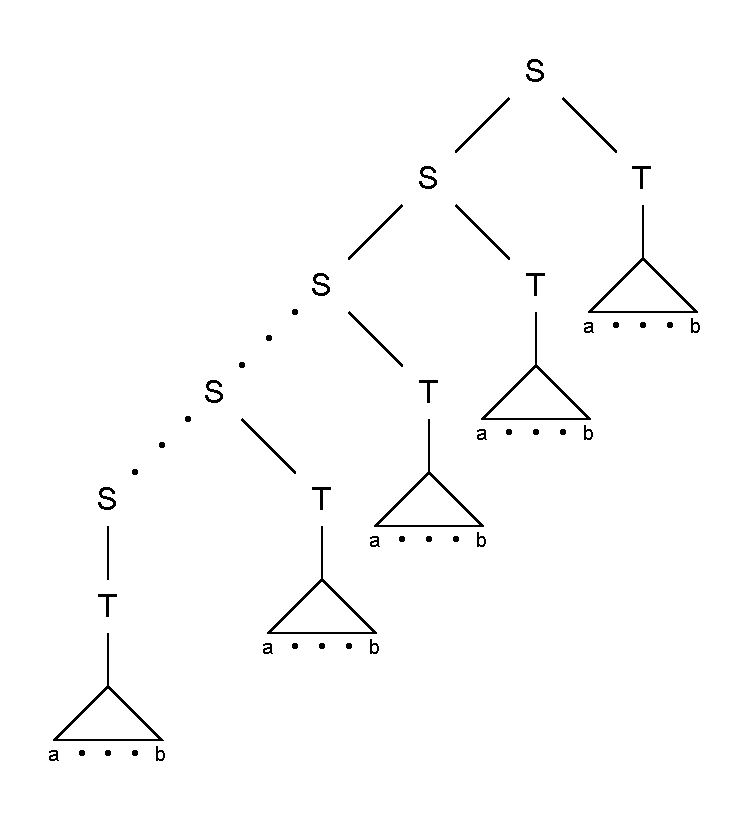
\includegraphics[scale=0.8]{Figures/Problem2.46b.pdf} \\
Structure of parse trees in $H$.
\end{center}
\end{proof}

\end{document}